\documentclass[11pt]{article}

\usepackage[margin = 1in]{geometry}

\usepackage{xcolor}
\definecolor{me}{HTML}{00a31b} %my comments are in green
\newcommand{\me}[1]{{\color{me} #1}}
\definecolor{highlight}{HTML}{ff0000}
\newcommand{\highlight}[1]{{\color{highlight} #1}}
\definecolor{gray}{HTML}{757c87}
\newcommand{\fade}[1]{{\color{gray} #1}}
\usepackage{graphicx}

\usepackage{tikz-feynman}

\usepackage{amsmath}
\usepackage{amsthm}
\usepackage{amsfonts}
\usepackage{slashed}

\newcommand{\defeq}{\ensuremath{:=}}
\newcommand{\corresponds}{\leftrightarrow}
\newcommand{\tr}{\operatorname{tr}}

\newcommand{\grp}[1]{\operatorname{#1}}
\newcommand{\lie}[1]{\mathfrak{#1}}
\newcommand{\vc}[1]{\mathbf{#1}}

\newcommand{\A}{\mathcal{A}}


\begin{document}

%!TeX root = ../main.tex 
\section*{Lecture 2, 18/01/2018}
\subsection*{Introduction}
\me{Throughout there was a lot of historiographic (what word is that for physics?) discussion that I didn't write down.}

Main topic for today is \emph{bosonization.}
We focus on $1+1$ relativistic dimensions although there are generalizations to other cases.
It is an equivalence between (certain classes of) bosonic and fermionic QFTs.

How is this possible, since bosonic theories have boson terms in their Lagrangians and fermionic ones have fermion terms?
Because theories aren't actually determined by their Lagrangians, but by their algebras of operators/correlation functions.

Bosonization is an example of a \emph{duality,} which are good for dealing with nonperturbative phenomena, especially to switch between strong and weak coupling.
Today we just work with free theories, however.

We \emph{will} turn on a self-coupling, and this turns our equivalence of free theories into ``sine-Gordon,'' which has a soliton excitation, \me{whatever that is.}
This is related to massless Schwinger theories (QED with massless fermions in $1+1$ dimensions.)

Apparently one of the people who worked on this was Elliott Lieb \me{who is the same person as the Temperley-Lieb algebra.}
A condensed matter application is to ``Luttinger liquids.''

\subsection*{The theory}
We work a free bosonic scalar field theory of a real-valued field $\phi$ with action
\[
S(\phi) = \int d^D x \left [ \frac{1}{2} (\partial \phi)^2 + V(\phi) \right]
\]
Here the integration measure is Wick rotated to Euclidean signature, even if we are interested in other signatures.
$V(\phi)$ is a potential term that includes masses, self-interactions, etc.
For now $V = 0$.
The partition function is
\[
\mathcal{Z} = \int \mathcal{D} \phi(x) e^{-S(\phi)}
\]
where the phase of the action in the integrand is chosen to make things converge nicely, and is the correct choice. \me{Apparently this was discussed either in the first lecture or last semester?}

The case $D = 2$ is special.
To see why, observe that the correlator
\[
\left \langle \phi(x) \phi(0) \right \rangle = \frac{\Gamma\left(\frac{D-2}{2}\right)}{\left( 4\pi\right)^{D/2}} \left( \frac{1}{x^2} \right)^{\frac{D-2}{2}}
\]
behaves poorly as $D \to 2$.
We will need both a UV and an IR regulator to fix this.

To derive the previous expression:
\begin{align*}
\int \frac{d^D k}{(2\pi)^D} \frac{e^{ikx}}{k^2} &= \int_0^\infty \int \frac{d^D k}{(2\pi)^D} \exp{-sk^2 + ikx}\\
&= \int_0^\infty ds \left( \sqrt{\frac{\pi}{s}} \right)^D \frac{\exp(-x^2/4s)}{(2\pi)^D}\\
&\me{\text{(change variables)}}\\
&= \frac{1}{2^D \pi^{D/2}} \int_0^\infty ds \;s^{D/2-1} \exp(-sx^2/4)\\
\end{align*}
which is equal to the original expression once you write it in terms of the gamma function.

This doesn't work for $D=2$.
To deal with that case we introduce an IR mass regulator $m_0 \ne 0$.
We also change the theory by making it $\phi$-periodic, i.e.~having $\phi$ take values in a circle with radius $R$.
This means that $\phi = \phi+ 2\pi$ and the action becomes
\[
S(\phi) = \frac{1}{g^2}\int d^2 x \left[ \frac{1}{2}(\partial \phi)^2 + \frac{1}{2} m_0 \phi^2 \right]
\]
where the ``coupling constant'' $g = R$ is the radius of the circle.
(It's still called a coupling constant even though it's not actually coupling anything.)

Now, the propagator is
\begin{align*}
G(\phi, m_0^2) &= g^2 \int \frac{d^2 k}{(2\pi)^2} \frac{e^{ikx}}{k^2 + m_0^2}\\
&\approx g^2\left( - \frac{1}{2\pi} \log m_0 + \text{const.} + \mathcal{O}(m_0|x|) \right)
\end{align*}
where $\approx$ means it's an asymptotic expansion.
We get a log divergence in $m_0$.
How do we deal with it?

One consequence: a massless field in $1+1$ dimensions doesn't exist as a quantum object, because of this IR divergence.
This means that there is never any spontaneous symmetry breaking in $1+1$ relativistic dimensions.
This result is the ``Coleman-Mermin-Wagener'' (sometimes also ``Hohenberg'') theorem.
It's really just the converse of Goldstone's Theorem, which says that in a relativistic QFT, if a continuous global internal (i.e.~not spacetime) symmetry is broken, there is a massless mode $\phi$.
In fact, such breaking and modes are in 1-1 correspondence.

If $\phi$ doesn't exist, how is this an interesting theory?
Well, we don't care about the Lagrangian, just the observables.
Even though correlators like $\langle \phi \phi \rangle$ are not well-defined, we still have things like
\begin{itemize}
    \item $\partial_\mu \phi$ and $\epsilon^{\mu \nu} \partial_\nu \phi$, which have to do with the conserved current of the $U(1)$ symmetry
    \item $V_\pm = e^{\pm i \phi}$, so-called ``vertex operators''
\end{itemize}
In particular, we can compute
\[
\left \langle V_+(x_1) \cdots V_=(x_n) V_-(y_1) \cdots V_-(y_m) \right \rangle
\]
at least if it exists when $m_0 \to 0$.
In order to do this we'll need to introduce a UV regulator $\Lambda$ and a corresponding renormalization group scale $\mu$.

For now, focus on the simple case $\langle V_+(x_1) V_-(x_2) \rangle$.
\me{I don't quite follow the details of the next calculation.}
This is a special case of
\[
\left \langle \exp \left( i \int d^2x\; J(x) \phi(x) \right) \right \rangle
\]
for some sourcelike term $J(x)$.
In this case it's $\delta^2(x_1) - \delta^2(x_2)$, so this can be rewritten using the propagator $G$ as
\[
\exp\left( -\frac{1}{2} \int d^2x d^2y\; J(x) G(x,y) J(x \me{\text{ or $y$?}})\right)
\]
where $J(x) = \delta(x_1) - \delta(x_2)$.

In this case this gives
\[
\langle V_+(x_1) V_-(x_2) = \exp\left( -\frac{1}{2} \cdot 2 G(0,m_0^2) + \frac{1}{2} \cdot 2 G(x_1 - x_2,m_0^2)\right)
\]
The first term is a problem on its face, because we'd get a UV divergence as $x \to 0$ in $\log m_0|x|$.
To fix this, we introduce a lattice spacing $a = 1/\Lambda$, which replaces the zero.

Only keeping the logarithmic terms, we then have
\begin{align*}
    \langle V_+(x_1) V_-(x_2) &= \exp \left( \frac{g^2}{2\pi} \left[ \log(m_0/\Lambda) - \log(m_0|x_1 - x_2|) \right]\right)\\
    &= \left( \frac{1}{|x_1 - x_2| \Lambda} \right)^{g^2/2\pi}
\end{align*}
The naive (``engineering'') scaling dimensions of of $\phi$ and $e^{i \alpha \phi}$ (for $\alpha \in \mathbb Z$) are both zero, which would cause problems.
Here quantum fluctuations save us by changing the scaling dimension to $g^2 /4\pi$.
This is an ``anomalous dimension $\gamma$.''

Now to deal with the UV cutoff.
Really the $V_\pm$ are the bare operators, which need to be renormalized.
We rewrite
\[
\left( \frac{1}{|x_1 - x_2| \Lambda} \right)^{g^2/2\pi} = \left( \frac{1}{\mu|x_1 - x_2| } \right)^{g^2/2\pi} \left( \frac{\mu}{\Lambda} \right)^{g^2/2\pi}.
\]
which helps because we can now define (notation used for historical reasons) $\sqrt{Z} V_{\pm}^R = V_\pm$, where
\[
\sqrt{Z} = \left( \frac{\mu}{\Lambda} \right)^{g^2/4\pi}.
\]
Now
\begin{align*}
\langle V^R_+ V^R_- \rangle = \left( \frac{1}{\mu |x_1 - x_2|} \right)^{g^2/2\pi}
\end{align*}
with $[V_\pm^R] = g^2 /4\pi \ne 0$.
We can now compare this to the free Dirac theory.


%!TeX root = ../main.tex 
\section*{Lecture 3, 23/01/2018}
Today we continue with the bosonic theory from last time and compute the correlator
\[
G^{(n,m)}_{\text{bare}} \defeq \left \langle V_+(x_1) \cdots V_+(x_n) V_-(y_1)\cdots V_-(y_m) \right \rangle
\]
As before we use a Gaussian with source a difference of $\delta$-functions:
\[
J = \sum_i \delta(x_i) - \sum_j \delta(y_j)
\]
In $J^2$ there are $n$-self contractions of $\delta(x_i)^2$, $m$ for the $y_j$, $n(n-1)$ of $x_i$ with a different $x_{i'}$, $m(m-1)$ for the $y_j$, and $nm$ $xy$ terms.
We get an overall factor
\[
G_{\text{bare}}^{(n,m)} \sim m_0^{n+m+n(n-1) + m(m-1) - 2nm} = m_0^{(n-m)^2}
\]
Thus in the $m_0 \to 0$ limit the correlators are zero unless $n=m$:
\[
G^{(n,m)} = m_0^{\frac{g^2}{2 \pi} (n-m)} \left( \frac{1}{\Lambda}\right)^{\frac{g^2}{4\pi} (n+m)} \left( \frac{\prod_{i\ne i'} |x_i - x_{i'}| \prod_{j \ne j'} |y_j - y_{j'}|}{\prod_{i,j} |x_i - y_j|}\right)^{\frac{g^2}{2\pi}}
\]

The nonzero case is a clue towards a symmetry.
In this case it's that the massless field $\phi$ has a global $U(1)$ symmetry given by $\phi \mapsto \phi + \text{const}$.
Furthermore, the renormalized propagator is
\[
G^{(n,n)}_{(R)} = \left( \frac{1}{\Lambda}\right)^{\frac{g^2}{2\pi} n} \left( \frac{\prod_{i\ne i'} \mu |x_i - x_{i'}|  \prod_{j \ne j'} \mu |y_j - y_{j'}|}{\prod_{i,j} \mu|x_i - y_j|}\right)^{\frac{g^2}{2\pi}}
\]
This is secretly a fermion theory.

The RG equation for this theory (a simple version of the Callan Symanzik equation) is
\begin{align*}
0 &= \mu \frac{\partial}{\partial \mu} \\
&= Z^n \left( \mu \frac{\partial}{\partial \mu}^{2n} + 2n \mu \frac{\partial \log \sqrt Z}{\partial \mu} \right) \left \langle V_+^{(R)} \cdots V_-^{(R)} \right \rangle\\
&= \left( \mu \frac{\partial}{\partial\mu} + 2n \frac{g^2}{4\pi}\right) G^{(n,n)}_{(R)}
\end{align*}
Compare to the general formula for dependence on the RG scale:
\[
\left( \mu \frac{\partial}{\partial \mu} + \beta(g) \frac{\partial}{\partial g} + n \gamma_+(g) + n \gamma_-(g) \right) G_{(R)}(x;\mu;g).
\]
Here $\mu$ is the scale, $g$ is a coupling constant, and $\gamma_\pm$ are the ``anomalous quantum dimension(s).''
In our case the beta function vanishes, so we get exact CFTs everywhere \me{in R(?)}
More generally, CFTs with central charge $c = 1$ have been completely classified; we will return to this later.

\subsection*{Fermionic theory}
We now work with free Fermions in $\mathbb{R}^{1+1}$, flat Lorentz spacetime Wick rotated to Euclidean signature.
To \emph{really} check equivalence we should examine other topologies, but we won't bother.
Maybe in a string theory course.

Below $\psi$ is a Dirac fermion.\footnote{We could use a pair of Majorana fermions, since those are equivalent in genus zero, but they aren't in other cases so we won't.}
We do the usual thing with $\psi = \begin{bmatrix} \psi_+ \\ \psi_- \end{bmatrix}$ and write the action as
\[
S(\psi, \bar \psi) = \int dz d\bar z \; \left( \bar \psi_+ \partial_{\bar z} \psi_+ + \bar \psi_- \partial_z \psi_-\right)
\]
This has a classical $U(1) \times U(1)$ symmetry parametrized by $\theta, \theta_5$:
\begin{align*}
\psi &\mapsto e^{i \theta +i \theta_5 \gamma_5} \psi\\
\psi &\mapsto e^{-i \theta +i \theta_5 \gamma_5} \psi
\end{align*}
where $\gamma_5$ is the \emph{third} gamma matrix and is called that in analogy with dimension 4.
The currents are
\begin{align*}
J_\mu &= \bar \psi \gamma_\mu \psi\\
J_\mu^5 &= i \bar \psi \gamma_5 \gamma_\mu \psi
\end{align*}
Since (depending on your $\gamma$ matrix conventions) $i \gamma_5 \gamma_\mu = - \epsilon_{\mu \nu} \gamma^\nu$ the currents are related to one another.

Now the propagators are 
\begin{align*}
\Delta^+ &= \left \langle \bar \psi _+(z,\bar z) \psi_+(0)\right \rangle = - \frac{1}{2\pi z}\\
\Delta^- &= \left \langle \bar \psi _-(z,\bar z) \psi_-(0)\right \rangle = - \frac{1}{2\pi \bar z}.
\end{align*}
Then (have to have the same number of $\psi$ and $\bar \psi$ terms)
\[
\left \langle \prod_{i=1}^n \bar \psi_+(z_i) \psi_+(z_i') = \left ( -\frac{1}{2\pi} \right)^n \det \left [ \frac{1}{z_i - z_j'}\right]_{ij} \right \rangle
\]
and similarly for $-$ but with $\bar z_i$ on the right-hand side.
\me{Here we wrote out expressions for $J_1$ and $J_2$ but I'm not sure why.}

Now, if we write $\sigma_+ = \bar \psi_- \psi_+$ and $\sigma_- = \bar \psi_+ \psi_-$, we find that their correlators are the same as in the bosonic theory.
Specifically, define $\varphi$ to be the same as $\phi$ but $R$-periodic \me{(instead of $2\pi$-periodic.)}
Then the map
\[
2 \pi \sigma_\pm \mapsto \mu \left[ e^{\pm i \sqrt{4\pi} \varphi} \right]_{(R)}
\]
is an equivalence
\begin{align*}
\bar \psi \slashed \partial \psi &\leftrightarrow \frac{1}{2} (\partial_\mu \varphi)^2\\
\bar \psi \gamma^\mu \psi &\leftrightarrow \frac{\varepsilon^{\mu\nu}}{\sqrt \pi} \partial_\nu \varphi \equiv j^\mu \sim \epsilon^{\mu \nu} \mathcal{J}_\nu
\end{align*}
\me{not sure what the stuff on the end is about.}
This is an ``electric-magnetic duality'' and can be compared to $T$-duality in a string theory context.

We can now start filling in a diagram of theories with ``one degree of freedom,'' which rigorously means CFTs with central charge $1$ (when parametrized correctly.)
Here's a partial chart, where $\#$ is some dimensionful constant \me{like string length.}
\begin{center}
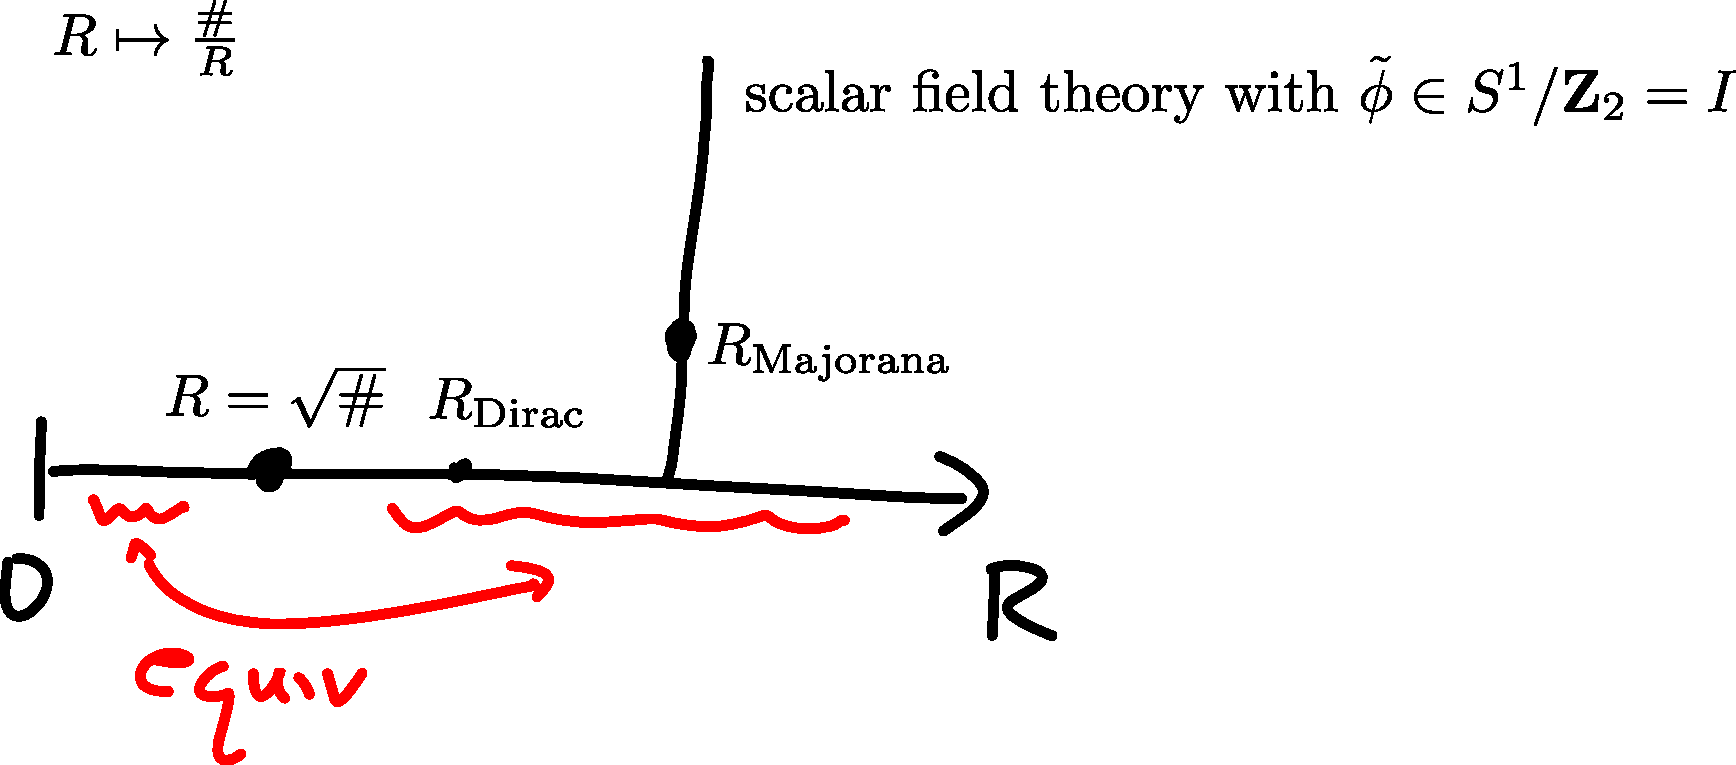
\includegraphics[width = 7in]{fig/lecture3CFTchart.pdf}
\end{center}






%!TeX root = ../main.tex 
\section*{Lecture 4, 25/01/2018}
\me{I missed the first 20 minutes but I think it was just review of last time.}

We previously computed
\begin{align*}
\left \langle \prod_1^n \sigma_+(x_i) \sigma_-(y_j) \right \rangle &= (-1)^n \left \langle \prod_1^n \bar \psi_+(y_i) \psi_+(x_i) \right \rangle\\
&= \left ( \frac{1}{2 \pi} \right)^{2n} \left [ \frac{ \prod_{i < j} |x_i - x_j|^2 |y_i - y_j|^2 }{ \prod_{i,j} |x_i - y_j|^2 } \right ]^{g^2/4 \pi}.
\end{align*}
To get this to match up, we need $g^2/4 \pi = 1$, so now we just set $g = \sqrt{4\pi}$.
The correlator above is supposed to be equal to
\begin{align*}
\left( \frac{1}{2 \pi}\right)^{2n} \left \langle \prod_{i = 1}^n \mu^2 V_+^{(R)}(x_i) V_-^{(R)}(y_i) \right \rangle,
\end{align*}
so we posit that
\begin{align*}
\sigma_\pm &= \mu V_\pm^{(R)}\\
V_\pm^{(R)} &= \left( \frac{\Lambda}{\mu} \right)^{g^2/4 \pi} V_\pm
\end{align*}
so that
\begin{align*}
\bar \psi_- \psi_+ &= \frac{\Lambda}{2 \pi} e^{i \phi}\\
\bar \psi_+ \psi_- &= \frac{\Lambda}{2 \pi} e^{-i \phi}
\end{align*}

Note that when defining $\varphi = \phi/g$ (choosing a canonical length scale) so that $\varphi = \varphi + 2 \pi$) we instead get $\bar \psi_- \psi_+ = e^{i \sqrt{4\pi} \varphi}$, etc.
This convention is in some (most?) literature.
More generally, the correspondence is
\begin{align*}
\bar \psi \slashed \partial \psi &\corresponds \frac{1}{2} (\partial_\mu \varphi)^2\\
j^\mu \defeq \bar \psi \gamma^\mu \psi &\corresponds \frac{\varepsilon^{\mu \nu}}{\sqrt \pi} \partial_\nu \varphi\\
\bar \psi \psi &\corresponds \Lambda \cos(\sqrt{4 \pi} \varphi)\\
\bar \psi \gamma^0 \gamma^1 \psi &\corresponds \Lambda \sin(\sqrt{4 \pi} \varphi)
\end{align*}
\me{The last was written using $\gamma_* \defeq \gamma^0 \gamma^1$ but this notation was not used again.}

\subsection*{Application one of bosonization}
Often we want to add a self-interaction density $\rho(x) V(x,y) \rho(y)$ to a theory.
This density $\rho$ is really $j^0$.
We now get a term $j^0 V j^0$ that is quartic in $\psi$, but bosonization lets you turn this in a term like $(\partial_0 \varphi)^2$, which is quadratic and therefore can be computed using a Gaussian.

\subsection*{Application two of bosonization}
Consider a simple $(1+1)$-dimensional condensed matter system, say a lattice model with operators $\psi(n), \psi^\dagger(n)$ on each vertex, with $\{ \psi^\dagger(n), \psi(m) \} = \delta_{m+n}$. 
(It's not immediately clear that this is relevant, since it's a non-relativistic system, but we'll get there.)
We use a Hamiltonian of the form
\[
H = - \sum_{n \in \mathbb Z} \psi^\dagger (n) \psi(n+1) + \text{h.c.}
\]
The Fourier transform of this is
\[
H = - \int_{-\pi}^\pi \frac{dk}{2 \pi} (\cos k) \psi^\dagger \psi
\]
where these $\psi$s are actually the momentum-space versions.

The ground state is a Fermi sea.
It looks like a graph of $- \cos$ on $[-\pi, \pi]$, and the 1-d excitations live near the zeros, at $\pm \pi/2$.
Zooming in it's a line with slope $c$, and the excitations move with $\omega = \pm ck$, where $k$ is the difference.
These are like free Dirac fermions.

In \emph{more} dimensions this doesn't quite work: you in general get a $(d-1)$-sphere of fermions, and for $d > 1$ this has infinitely many points, which is hard to deal with.

\subsection*{Massless Schwinger model}
Here the action is (expanding out the gauge derivative $\slashed D$) is
\[
S = \int d^2 x \left[ \bar \psi \slashed \partial \psi + A_\mu j^\mu - \frac{1}{4 e^2} F_{\mu \nu}F^{\mu \nu}\right],
\]
where we put the electric charge $e$ with the $F^{\mu \nu}$ term to match the usual conventions for a Yang-Mills theory.
This theory is potentially complicated because of the interaction terms: you get \emph{lots} of Feynman diagrams.
However there are simplification.

In two dimensions, the $\beta$ function is dimensionful, so the theory is superrenormalizable, i.e.~free in the UV limit.
Another interesting feature is that there are zero polarizations (compare $3-1 = 2$ in reality), bt least classically.
When we quantize we'll get new things and the theory won't be trivial.

To solve the theory we use the correspondence $\psi \bar \psi \corresponds \varphi$ \me{the $\psi$ term looks wrong here} to change the action to
\[
S = \int d^2 x \left [ \frac{1}{2} (\partial_\mu \varphi)^2 + \frac{\partial_\mu \varphi}{\sqrt \pi} \partial^\mu f + \frac{1}{2e^2} \partial^2 f \partial^2 f\right],
\]
where we have written $A_\mu = \partial_\mu \alpha + \varepsilon_{\mu \nu} \partial^\mu f$ and (locally) gauge transformed $\alpha = 0$.
We work in Minkowski signature, so that $\varepsilon_{01} = 1$, $\eta_{00} = 1$, $\eta_{11} = -1$, $\varepsilon^{01} = -1$, and $\varepsilon_{\mu \nu} \varepsilon^{\nu \sigma} = \delta_\mu^{\phantom{\mu} \sigma}$.

Notice that we have turned a cubic self-interaction into a quadratic term!
This is a \emph{free} bosonic theory.

Actually, we should also integrate by parts to change the middle term to $- \frac{\varphi}{\sqrt \pi} \partial^2 f$, so that
\begin{align*}
S &= \int d^2 x \left[ - \frac{1}{2 \pi} \partial_\mu f \partial^\mu f + \frac{1}{2e^2} \partial^2 f \partial^2 f\right]\\
&= \int d^2 x \left[ \frac{1}{2 \pi} A_\mu A^\mu + \frac{1}{2e^2} A_\mu \partial^2 A^\mu\right]
\end{align*}
\me{I don't really get what's happening here.}

The result is a theory of a propagating scalar with
\[
\left \langle A_\mu A_\nu \right \rangle = \left( \eta_{\mu \nu} - \frac{p_\mu p_\nu}{p^2} \right) \frac{1}{p^2 - e^2/\pi}
\]
with corresponding dispersion relation $\omega^2 = k^2 + e^2/\pi$.
The two-point function has no cuts, just poles, so we get \emph{confinement:} there are no asymptotic states with charge.

``Spontaneous breaking of chiral symmetry'' \me{is a phrase stated at the end of class.
It may be related to
\[
\langle \sigma_\pm \rangle = \frac{\Lambda}{2 \pi} \langle e^{\pm i \theta} \rangle
\]
and a new scalar field $\theta$.
Apparently in the above the $\Lambda$s cancel.}

%!TeX root = ../main.tex 
\section*{Lecture 5, 30/01/2018}
We discussed the bosonization correspondence from before, and returned to the chart of relativistic CFTs with ``one degree of freedom'' in $1+1$ dimensions.
Main new comment was that it follows an ADE classification: the two axes are the A and D and the E refers to the three isolated theories.
The reason for this has to do wtih classifying the discrete subgroups of $\operatorname{SU}(2)$.

\subsection*{Thirring and sine-Gordon}
``Sine-Gordon'' is a pun on ``Klein-Gordon'' since there's a (co)sine in it.
The action is
\[
S_{\text{SG}} = \int d^2x \left [ \frac{1}{2} \partial_\mu \varphi \partial^\mu \varphi + \frac{m^4}{\lambda} \cos\left ( \frac{\sqrt \lambda}{m} \varphi\right ) \right ]
\]
Here $m$ is the mass and $\lambda$ is the self-coupling.
The $m^4$ is the right thing to do for a theory in $1+1$ dimensions.
Sometimes there's a $1$ subtracted from the cosine to make the theory have $\varphi = 0$ give zero energy, but absolute energy levels don't matter so we drop it.
This theory is integrable both clasically and on a quantum level.

The equation of motion is
\[
\partial^\mu \partial_\mu \varphi + \frac{m^2}{\lambda} \sin \left(\frac{\sqrt \lambda }{m} \varphi \right)
\]
which has infinitely many zero-energy solutions because of the periodicity.
We could do perturbative expansion around each one and they wouldn't interact, because it's not possible to jump between wells like that in infinite space.
\me{There was a comment about that being true clasically but not when we quantize but I'm not sure what the actual statement is.}

Instead we quantize a \emph{soliton}, which for our purposes means a thing that doesn't dissipate, usually associated to a conserved quantity.
Once we have one we can boost it to any velocity \me{and quantize around these.}

Define $\bar x = mx$, $\bar t = mt$, $\bar \varphi = \frac{\sqrt \lambda}{m} \varphi$.
We have symmetries $\bar \varphi \mapsto - \bar \varphi$, $\bar \varphi \mapsto \varphi + 2\pi$.
If $\bar \varphi (- \infty ) = 2 \pi N_1$ and $\bar \varphi(\infty) = 2 \pi N_2$, then we get a ``topological charge''
\[
Q = N_1 - N_2 = \frac{1}{2 \pi} \int d \bar x \partial_{\bar x} \bar \varphi \sim \int d \bar x j^0
\]
Note that $\varphi \mapsto \varphi + c$ is \emph{not} a symmetry of the theory.

For $Q = \pm 1$ we get soultions
\[
\bar \phi (x) = \pm 4 \operatorname{atan} e^{-\bar x - \bar x_0}
\]
which we call solitons and antisolitions.
\me{(Many of the formulas here may be wrong.)}
They have scattering
\[
4 \operatorname{atan} \left( \frac{\sinh(u \bar t/ \sqrt{1-u}) }{u \cosh(\bar x \sqrt{1-u^2}) } \right).
\]
\me{Under $u \mapsto iv$??} we get ``breather'' or ``doublet'' solutions
\[
\bar \phi = 4 \operatorname{atan}\left[ \frac{\sin(\pi \bar t/\sqrt{1+v^2})}{v \cosh (\bar x /\sqrt{1+v^2})}\right]
\]
Also, the energy of the classical solution is $8m^3/\lambda$, while the energy of the quantum solution is $8m^3/\lambda + m/\pi + \mathcal{O}(\lambda).$ \me{There was a comment about the importance of that that I missed.}

We return to the original model to bosonize. With $\phi = \frac{\sqrt{\lambda}}{m} \varphi$, we have
\[
S_{\text{SG}} = \frac{m^2}{\lambda} \int \frac{1}{2} (\partial_\mu \phi)^2 + m^2 \cos \phi
\]
The coupling constant $g$ from before is now usually called $\kappa$, with $\kappa^2 = \lambda/m^2$.
The proof \me{of the following (?)} is careful and order-by-order but we don't discuss it.

The Thirring model is
\[
S_T = \int d^2 x \left[\bar \psi (\slashed \partial + m_F) \psi - \frac{1}{2} g J_\mu J^\mu \right].
\]
When bosonizing: the $\slashed \partial$ term becomes $(\partial_\mu \varphi)^2$, the $m_F$ term becomes $\Lambda \cos \varphi$, and the final term gets two $\varepsilon^{\mu \nu}$s, which combine to give an $\eta^{\mu \nu}$, so it becomes $(\partial_\mu \varphi)^2 g / \pi$.
We have thus shown that
\[
1 + \frac{g}{\pi} = \frac{4\pi}{\kappa^2}
\]

Implications:
\begin{itemize}
    \item The fermion mass $m_F$ is zero \me{(?)}
    \item The sine-Gordon theory can be shown to be non-renormalizable, so we've shown that Thirring isn't either, which would have been much harder directly.
    \item The fermion $\psi$ corresponds to the soliton in the sine-Gordon theory.
\end{itemize}

In the next lecture, we will discuss quantization of (non-abelian) Yang-Mills theories.

%!TeX root = ../main.tex 
\section*{Lecture 6, 01/02/2018}
Today we discuss Yang-Mills theories, for now in Minkowski spacetime of $3+1$ dimensions.

In 1954 QED was figured out, which is a theory of a potential $A_\mu$ and fields $\psi$, $\phi$, etc.
It was very succesful, and used an \emph{abelian} $\grp U (1)$ gauge symmetry.
Attempts to generalize this to non-abelian gauge groups were considerably more difficult, and this is what we explain now.

Recall that for a scalar field $\phi(x)$, gauge invariance requires us to promote $\partial_\mu$ to a \emph{covariant derivative}
\[
D_\mu(A) \defeq \partial_\mu - i e A_\mu.
\]
This results in a $U(1)$ invariant theory and automatically includes self-interactions of the gauge field $A_\mu$.

We now promote $\phi$ to a vector $\phi^i$ and the symmetry group to $\grp U(N)$ (or some other compact Lie group $G$.)
Now the transformation $\phi(x) \mapsto U \phi(x)$ is a symmetry of the action
\[
S = \int \partial \bar \phi \partial \phi \pm m^2(\bar \phi \phi) + \frac{\lambda}{\text{numerical constant}} (\bar \phi \phi)^2
\]
This is an invariant ``global'' symmetric because it acts on all of spacetime in the same way.
It could be ``broken,'' which means that the vacuum state is not preserved by the charges ($Q \left | 0 \right \rangle \ne 0$.)
If it isn't, we get an actual symmetry acting on the states.

We now want to ``gauge'' this symmetry by promoting it to a ``local'' symmetry
\[
\phi(x) \mapsto U(x) \phi(x)
\]
For this to work we need a \emph{covariant} derivative.
Observe that
\[
\partial_\mu(U \phi) = U \partial_\mu \phi + (\partial_\mu U) \phi = U(\partial_\mu \phi + (U^{-1} \partial_\mu U)) \phi,
\]
so we postulate
\[
D_\mu \phi^i(x) = \partial_\mu \phi^i - i A_\mu^{ij}(x) \phi^j(x)
\]
where now $A_\mu$ is ``matrix-valued,'' taking values in the adjoint representation of the gauge group $G$, which is to say in its Lie algebra $\lie g$.
Notice that we've absorbed the charge into $A_\mu$, which is more convenient right now, although we'll want it back when we do perturbative calculations.
In this convention, $[A_\mu] = [\partial_\mu] = 1$, which is convenient.

\me{Here there was a brief discussion of Lie theory: $\lie g = T_eG$, the exponential map, the Killing form, etc.
I already knew about this so I didn't write it down, but there was a mention of Zee's book on group theory as a good reference.}
We will only work with compact gauge groups $G$ for now, although we might allow non-compact ones later when we talk about Chern-Simons theories.
Note that physicists frequently forget about $\lie g$ and just call everything $G$.
We work in a basis $T^a$ of $\lie g$ that diagonalizes the Killing form.

Now, under the group transformation $e^{i \theta^a(x) T^a}$ the gauge field transforms as
\[
A_\mu \mapsto A_\mu + i \theta^a [T^a, A_\mu] + \partial_\mu \theta^a T^a.
\]
In the previous case of QED the middle term vanishes.
There are some divergent conventions here with the factors of $i$.
It has to do with what goes in the exponential: physicists like an extra factor of $i$ so that the Lie algebra is Hermitian.
Therefore in physics
\[
[T^a, T^b] = i f^{ab}_{\phantom{ab}c} T^c,
\]
while in math there's no $i$.
In any case, the structure constants are antisymmetric in the first two indices.
In the physics convention, note that we can write
\[
A_\mu^a \mapsto A_\mu^a + \partial_\mu \theta^a - f^{abc} \theta^b A_\mu^c
\]
In fact, for \emph{compact} Lie groups $f^{abc}$ is always fully antisymmetric.
In the particularly simple case of $\grp{SU}(2)$, $f^{abc} = \varepsilon^{abc}$.

We call $A_\mu^a$ a ``gauge field.''
Really, it's a local representation of a connection on a $G$-principal bundle.
\me{Here there was a discussion of $G$-principle bundles that I again didn't write down.}
Note that we treat gauge symmetries rather differently than regular ones: they are \emph{redundancies} in our descriptions of the fields, not transformations between physically different states.

Another change: In QED, $F_{\mu \nu}$ was invariant.
In general it will just be covariant:
\[
F_{\mu \nu} \mapsto U^{-1}F_{\mu \nu} U
\]
If we view $A = A_\mu dx^\mu$ as a matrix-valued $1$-form, then it transforms as
\[
A \mapsto U AU^{-1} + U dU^{-1},
\]
and we define $F$ by
\[
F = dA + A \wedge A.
\]
Recall of course that the wedge product of Lie-algebra valued forms involves using the bracket to contract things.
Then in terms of components,
\begin{align*}
F^{\text{math}}_{\mu \nu} &= \partial_\mu A_\nu - \partial_\nu A_\mu + [A_\mu, A_\nu]\\
F^{\text{physics}}_{\mu \nu} &= \partial_\mu A_\nu - \partial_\nu A_\mu - i[A_\mu, A_\nu]
\end{align*}
Before adding in matter, our Yang-Mills action is now
\[
S_{\text{YM}} = \frac{1}{-2g^2_{\text{YM}}} \int d^4x\, \tr(F_{\mu \nu} F^{\mu \nu})
\]
Here the trace is really the Killing form, with the choice $\tr(T^a T^b) = \delta^{ab}/2$.
This is also related to the normalization of the coupling constant.
Even before adding in matter this theory is self-interacting: we get diagrams like
\begin{center}
\feynmandiagram [inline =(e.base)] {
    a -- [photon] e,
    b -- [photon] e,
    c -- [photon] e,
};
and 
\feynmandiagram [inline =(e.base), horizontal = a to b] {
    a -- [photon] e,
    b -- [photon] e,
    c -- [photon] e,
    d -- [photon] e,
};
\end{center}

Recall that in QED the Gaussian term wasn't invertible.
Therefore, to get the propagator we just guessed that
\[
\left \langle A_\mu A_\nu \right \rangle \sim \frac{\eta_{\mu \nu}}{p^2 + i \varepsilon}
\]
and checked that it worked.
In fact, it only does because the matter fields are coupled to a conserved current: if not we'd need an extra term $p_\mu p_\nu/p^2$ in the numerator.
More generally, this only works because the QED $S$-matrix is unitary.

In Yang-Mills the $S$-matrix is \emph{not} unitary, so this method doesn't work.
This was a major theoretical problem.
It was eventually solved by Faddeev and Popov by carefully working through the Hamiltonian formalism.
%!TeX root = ../main.tex 
\section*{Lecture 7, 06/02/2018}
We continue with the quantization of Yang-Mills theories.
\me{While reviewing some notation, there was a discussion of the classification of these theories that I missed.
A big part of the classification is just the classification of semisimple Lie groups.
There was also some mention of ``topological terms'' like $\tr(F \wedge F).$}

Physicists confusingly sometimes call $\grp U(1)$ a simple Lie group and sometimes don't.
\me{I asked, and the lecturer had never heard of ``reductive,'' which is the correct term.}
We will not.
There is a classification theorem: all semisimple Lie groups \me{(which is defined to include simply connected)} are products of simple ones, which are in turn classified in series $A_n, B_n, C_n, D_n$ and the exceptional cases $E_6, E_7, E_8$, $F_4$, $G_2$.
\me{There was more discussion of this and some explanation, but I'm familiar already so I didn't write it down.
The reccommended physics reference is Zee's group theory book.
For math I like Fulton and Harris.}

To discuss quantization we follow Faddeev and Slavnov.
There is a path integral
\[
\mathcal Z = \int \mathcal D A_\mu \exp \left[\frac{i}{8g^2} \int \tr F_{\mu \nu}F^{\mu \nu}\right],
\]
which as usually completely fails to converge.
What this actually means is a shorthand for quantization in the Hamiltonian formalism.
Of course, there's a problem because we want to do Lagrangian things, which requires the ability to guess the answer.
This is part of the reason figuring out non-Abelian gauge theory was difficult.

From now on, we distinguish $\mathcal A_\mu \defeq A_\mu^a T^a$ from regular $A_\mu$, and similarly for $\mathcal F_{\mu \nu}.$
Under a gauge transformation $\omega$,
\[
\mathcal A_\mu \mapsto \mathcal A_\mu^\omega = \omega(x) \mathcal A_\mu \omega(x)^{-1} + \partial_\mu \omega(x) \omega(x)^{-1}
\]
Sometimes this will require putting indices in the wrong places so we can decorate with $\omega$.

The equations of motion are now
\[
\nabla^\mu \mathcal F_{\mu \nu} = 0,
\]
where $\nabla_\mu = D_\mu$.
However, there is a redundancy here, because $\nabla^\mu \nabla^\nu \mathcal F_{\mu \nu} = 0$ automatically.
This is related to the difficulty in dealing with terms like $A_\mu \mathcal O^{\mu \nu} A_\nu$ when $\mathcal O$ is not an invertible operator.

\subsection*{Hamiltonian form}
Observe that the Lagrangian (after rescaling to absorb the coupling constant)
\[
\tr \left( \left( \partial_\mu \mathcal A_\nu - \partial_\nu \mathcal A_\mu + g[\mathcal{A}_\mu , \mathcal A_\nu] - \frac{1}{2} \mathcal F_{\mu \nu}  \right) \mathcal F^{\mu \nu} \right)
\]
is up to a total derivative equal to 
\[
- \frac{1}{2} \tr \left( E_k \partial_0 \mathcal A_k - \frac{1}{2} (E_k^2 + G_k^2) + \mathcal A_0 \mathcal C\right)
\]
where $E_k = \mathcal F_{k0}$, $G_k = \frac{1}{2} \varepsilon^{ijk} \mathcal F_{ji}$, and $\mathcal C = \partial_k E_k - g[\mathcal A_k, E_k]$, $\mathcal C = C^a T^a$.
This is still a Lagrangian but at least \emph{looks} more like a Hamiltonian theory.
In particular $E_k^a, A_k^a$ are a canonical pair and $h = \frac{1}{2}[ (E_k^a)^2 + (G_k^a)^2]$ looks like a Hamiltonian.

This is a ``degenerate Lagrangian'' because the $q_I, p^I$ don't form a coordinate system in phase space; this has to do with the $\mathcal A_0$ term \me{i.e. gauge fixing (?)}
To deal with this, we follow Dirac and introduce constraints.

Note the Poisson brackets
\begin{align*}
\{ E_k^a(\vc x), A_l^b(\vc y)\} &= \delta_{kl} \delta^{ab} \delta(\vc x - \vc y)\\
\{C^a(\vc x), C^b(\vc y)\} &= g f^{abc} C^c(\vc x) \delta(\vc x - \vc y)
\end{align*}
say that we have a ``generalized Hamiltonian system.''

Compare this to the case of a classical system $\Gamma$ with $n$ degrees of freedom, so that phase space is $2n$-dimensional with coordinates $p_i, q^i$.
The action is
\[
S = \int \sum_i p_i \dot q^i - h(p,q) - \sum_a \lambda^a \phi^a(p,q) \, dt
\]
where the $\lambda$ are Lagrange multipliers and the $\phi$ are constraints.

To deal with this, we will want $\Gamma$ to have ``first-class constraints'', which means:
\begin{enumerate}
    \item[0.] \me{already assumed} $p$ and $q$ have canonical Poisson brackets
    \item $\{h, \phi^a\} = C^{\alpha \beta} (p,q) \phi^\beta$ 
    \item $\{\phi^a, \phi^b\} = C^{\alpha \beta \gamma} (p,q) \phi^\gamma$
\end{enumerate}
We will see next time that Yang-Mills is an example of such a system (with infinitely many degrees of freedom.)
%!TeX root = ../main.tex 
\section*{Lecture 7, 08/02/2018}
Today we discuss Hamiltonian quantization of Yang-Mills theories.
Why do we focus on the Hamiltonian picture?
Because it's easier to make sense of the path integral/partition function:
\begin{align*}
\mathcal Z &= \int \mathcal D q(t) \exp \left[i \int dt\, \mathcal{L}(q, \dot q, t)\right]\\
&= \int \mathcal D p(t) \mathcal D q(t) \exp \left[ i\int dt\, p\dot q- H \right]
\end{align*}
where heuristically $\mathcal L = p \dot q - H.$
The advantage here is that we have a canonical measure on the phase space, namely the standard symplectic form \me{for a cotangent bundle.}

In our case, we have
\begin{align*}
\mathcal L = E_k^a \partial_0 A_k^a - h(E_k , A_k) + A_0^a C^a
\end{align*}
where $E_k^a, A_k^a \sim p_i, q^i$ and $h = \frac{1}{2} [(E)^2 + (G)^2]$.
We can think of the $C^a$ as constraints.
The reference on quantization with constraints is Teitelboim \& Henneaux.

Re call that we are in a $2n$-dimensional phase space $\Gamma$ with action
\[
S = \int \sum_i p_i q^i - h(p,q) - \sum_{\alpha = 1}^m \varphi^\alpha(p,q)
\]
where $m < n$ because each one will kill two degrees of freedom.
These are ``first-class constraints,'', which are easier to deal with than other situations.

To quantize this: \me{(I think I missed many of the details, so this section may contain more errors than usual.)}
\begin{enumerate}
    \item Pick $m$ additional conditions (complimentary to the $\varphi$)
    \[
    \chi^\alpha(p,q) = 0
    \]
    satisfying
    \[
    \det [ \{ \varphi^\alpha, \chi^\beta\}]_{\alpha \beta} \ne 0
    \]
    and $\{\chi^a, \chi^b\} = 0.$
    \item Set $\chi^\alpha = 0$, $\varphi^\alpha = 0$ to get a $2(n-m)$-dimensional space $\Gamma^*$.
    \item Find canonical coordinates $p^*, q^*$ on $\Gamma^*$ satysifying
    \begin{align*}
    q &= (\chi^\alpha, q^*)\\
    p &= (p^\alpha, p^*)
    \end{align*}
    where the $p^\alpha$ are canonically conjugate to the $\chi^\alpha$.
    We then define
    \[
    h^*(p^*,q^*) = h(p,q)|_{\varphi = 0, \chi = 0, p^\alpha = p^\alpha(p^*,q^*)}
    \]
\end{enumerate}

\me{There was now a discussion of the equivalence of the new and the original equations of motion, but I didn't follow it and I think it was farily incomplete anyway.
I guess we'll just have to take it on faith.}

We can now interpret the path integral for the original system $\Gamma$ as the path integral for the constrained one $\Gamma^*$:
\[
\mathcal Z = \int \mathcal D p^*(t) \mathcal D q^* (t) \exp \left[ i \int p^* \dot q^* - h^*(p^*,q^*)\right].
\]
We claim that this is the same as
\[
\mathcal Z = \int \mathcal D p(t) \mathcal D q(t) \mathcal D \lambda(t) \prod_{t, \alpha} \delta(\chi^\alpha) \prod_t \det \left[\{ \varphi_\alpha , \varphi_b\} \right] \exp \left[ i \int p \dot q - h(p,q) - \lambda^\alpha \varphi(p,q) \right].
\]
The critical peice here is the determinant term, usually called a \emph{Faddeev-Popov determinant.}
For a long time people left this out when trying to quantize non-abelian Yang-Mills and it caused lots of problems.
It's essentially the Jacobian of the coordinate change.

\begin{proof}
The idea is to integrate out the $\lambda(t)$.
This has something to do with passing to a different system of coordinates?
All we need is to show that
\[
\delta(\chi^\alpha)\prod \det[\{\varphi_\alpha,\varphi_\beta\}] = \prod \delta(q_\alpha) \delta(p_\alpha - p_\alpha(p^*,q^*))
\]
and while this apparenlty seemed obvious when the notes were written, why this is actually true wasn't apparent. \me{We might fix this later?}
\end{proof}

Now we apply this to Yang-Mills (which we know from last time is of the first class.)
In order to do this we will have to temporary break Lorentz symmetry in order to gague fix.
We choose Coulomb gauge $\partial_k A_k = 0$, although other choices are reasonable.
We can check that
\begin{align*}
\{ \delta_k \mathcal A_k, \partial_i \mathcal A_i\} &= 0\\
\{C^a(\vc x), \partial_k A_k^a(\vc y) \} &= - \partial_k \left[\partial_k \delta^{ab} - g f^{abc} A^c_k(\vc x) \right]\delta(\vc x - \vc y)
\end{align*}
We call the operator in brackets \me{(maybe also with the $\partial_k$ on the left?)} $M_C[\mathcal A]$.
It is the critical part.
In the abelian case it's just the Laplacian, but since $G$ is non-abelian the second term doesn't vanish.

Now the partition function is
\[
\mathcal Z = \int \mathcal D A_\mu^a(x) \exp \left[ i \int d^4x \frac{1}{8} \tr\left(\mathcal F_{\mu \nu} \mathcal F^{\mu \nu}\right )\right]\prod \delta(\partial_k \mathcal A_k) \prod \det M_C[\mathcal A].
\]
How do we compute this determinant?
We introduce ``ghost'' and ``antighost'' variables $c(x)$, $b(x)$ (which is sometimes called $\bar c(x)$ because in a YM context it's the complex conjugate.)
These are ``Grassman'' variables that anticommute.
The point of doing this is that now
\[
\det M_C[\mathcal A] = \int \mathcal D c(x) \mathcal D b(x) \exp \left[ i \int d^4x\, b(x) M_C[\mathcal A]c(x) \right].
\]

Side note:
A simple analogy to our situation is the evaluation of the Gaussian integral
\[
\int dx\,dy\; e^{-(x^2 + y^2)} = \frac{1}{2\pi} \int dr \; r e^{-r^2}
\]
We can interpret this as the ``gauge fixing of a $U(1)$-invariant integrand,'' so that the denominator is the volume of the gauge group.
However, the inclusion of the Jacobian factor here is very important; you can't just divide by the volume.
\me{Also, the factor isn't $1/2 \pi$, it's $1/2$, so I'm not sure what mistake I made.
There was also a comment about how you can't just divide by $\int dy$ since that diverges.
The point might have been choosing the right coordinates?}
%!TeX root = ../main.tex 
\section*{Lecture 9, 13/02/2018}
A correction from last time: The Faddeev-Popov determinant should actually be
\[
\prod \det[ \varphi^\alpha, \chi^\beta]_{\alpha \beta}
\]
with a phi and a chi, not two phis.

\me{There was a recap of last time that I mostly missed.}

To apply the FP path integral to Yang-Mills, we could try to use Lorentz gauge $\partial^\mu A_\mu^a = 0$ (which is Lorentz-invariant) but this worn't work, and we instead need to use Coulomb gague $\partial_k A_k^a = 0$.

Now the partition function is
\[
\mathcal Z = \int \mathcal D E_i^a(x) \mathcal D A_\mu^a(x) e^{\frac{i}{8 g^2_{\text{YM}}} \int d^4x\, \tr(F_{\mu \nu} F^{\mu \nu}) } \prod \delta(\partial_k \mathcal A_k) \prod \det M_C[\mathcal A]
\]
We can now preform a Gaussian integral of the $E_i$ to get rid of one integration variable.

The ``matrix'' $M_C$ is
\[
M_C = \Delta \delta^{ab} - g f^{abc} A_k^a \partial_k
\]
This is the analogue of \me{$\partial_\mu \partial_\nu$ (or something like that, I missed this)} for $\phi^4$ theory.
Notice that the matrix depends on $\mathcal A$.

The big difference from QED is that there, while strictly speaking the matrix term should have appeared in the path integral, it doesn't depend on $\mathcal A$.
Therefore it just gives an overall constant which can be safely ignored.
This is \emph{not} the case for non-Abelian gauge theories.
Another way to avoid this determinant is to choose exactly the right gauge-fixing condition; we will return to this later.

How are we going to pass from Coulomb to Lorentz gauge in our path integral?
We use the ``Faddeev-Popov trick.''
Define
\[
\Delta_L(\mathcal A) \int \prod \delta(\partial_\mu \mathcal A_\mu^\omega) d \omega = 1
\]
where $\Delta_L(\mathcal A)$ will wind up being the FP determinant; for now it's defined by the above equation.
Here $\mathcal A_\mu^\omega$ (which should really have the $\mu$ upstairs) is the field $\mathcal A$ gague-transformed by the transformation $\omega$, and $d \omega$ is the invariant measure on the group $G$.
\me{Since $ \omega \in \Omega^1(G,\lie g)$ I assume this means the promotion of the measure to that infinite-dimensional group?}

An important fact here is that $\Delta_L(\mathcal A)$ is gauge invariant:
\[
\Delta_L(\mathcal A^{\omega'})^{-1} = \int \prod \delta(\partial_\mu \mathcal A_\mu^{\omega' \omega}) d \omega
\]
and this will wind up dropping out when we change variables to $\tilde \omega \defeq \omega' \omega$ in the integral, since the measure is invariant.

Notice that on the Coulomb condition surface,
\[
\prod \det M_c[\mathcal A] = \Delta_C(\mathcal A)
\]
\begin{proof}
Whenever $\partial _k \mathcal A_k = 0$, $\omega = e$ is always a solution of the $\delta$-function in the determinant.
If we concentrate on infinitesimally nearby solutions $\omega(x) \approx e + u(x)$, then
\[
\partial_k \mathcal A_k^\omega = \square u - g [\mathcal A_k, \partial_k u] = M_C[\mathcal A]
\]
\end{proof}

Now, we can change variables in the path integral from $\mathcal A_\mu$ to $\mathcal A_\mu^{\omega^{-1}}$:
\[
\mathcal Z = \int \mathcal D \mathcal A_\mu(x) \Delta_L(\mathcal A) \highlight{\int} \prod \delta(\partial_\mu \mathcal A_\mu) \highlight{d \omega} e^{\frac{i}{8 g_{\text{YM}}^2} \int d^4x\, \tr(F_{\mu \nu}F^{\mu \nu})} \highlight{\prod \delta(\partial_k \mathcal A_k^{\omega^{-1}}) \Delta_C(\mathcal A)}
\]
and all the terms in red will cancel.

The resulting Lorentz-invariant path integral is
\[
\mathcal Z = \int \mathcal D \mathcal A_\mu(x) \Delta_L(\mathcal A) \prod \delta(\partial_\mu \mathcal A_\mu)  e^{\frac{i}{8 g_{\text{YM}}^2} \int d^4x\, \tr(F_{\mu \nu}F^{\mu \nu})}.
\]
We got this by the trick of integrating only over the \emph{solution space} to the gauge-fixing conditions and adding in a determinant to deal with the ``coordinate change.''

To get the Feynman rules for this path integral we need to deal with the determinant and $\delta$-function terms.
We do this by
\begin{enumerate}
    \item Introducing a new auxiliary field $B^a(x) \defeq \partial^\mu \mathcal A_\mu^a$ and integrating over all choices:
    \[
    \int \mathcal D B^a(x) \cdots \prod (\partial_\mu \mathcal A^\mu - B) e^{i \int \cdots + i \xi \int \tr(B^2) d^4x}
    \]
    \item Introducing ghosts and antighosts to write
    \[
    \det M_C(\mathcal A) = \int \mathcal D b(x) \mathcal D c(x) e^{i \int d^4x\, bM_c(\mathcal A) c}
    \]
\end{enumerate}
These are not ``real'' particles, just a way to write down the determinant.
We will be more precise about this when we introduce BRST.

In summary (setting $g_{\text{YM}} = 1$) we have
\[
\mathcal Z = \int \mathcal D A_\mu(x) \mathcal D b(x) \mathcal D c(x) \mathcal D B(x) \exp\left[i \int d^4 x \frac{1}{8} \tr(F_{\mu \nu} F^{\mu \nu}) + \xi \tr(B^2) + i b M_c(\mathcal A)c \right] \delta(\partial_\mu \mathcal A^\mu - B)
\]
Here $B$ is an ``auxiliary field.''
When you get it out you get a $\tr(\partial_\mu \mathcal A^\mu)$ term that depends on $\xi$, the ``gauge-fixing parameter.''

This theory now gives Feynman rules, because even if the ghosts are strange nonphysical particles, there is no left-over gauge symmetry.
We can also now couple to matter fields $\phi, \psi, \dots$ corresponding to representations of $G$.
The propagators are:

\begin{align*}
&\text{gluons: } & \frac{i}{p^2 + i \varepsilon} \left[ -\eta^{\mu \nu} + (1- \xi) \frac{p^\mu p^\nu}{p^2}  \right] \delta^{ab} &= 
\feynmandiagram [horizontal = a to b, baseline = (a.base)] {
    a [particle = ${}^a_\mu$] -- [gluon] b [particle = ${}^b_\nu$]
};\\
&\text{ghosts: } & \frac{i \delta^{ab}}{p^2 + i \varepsilon} &= 
\feynmandiagram [horizontal = a to b, baseline = (a.base)] {
    a [particle = ${}^a$] -- [ghost] b [particle = ${}^b$]
};\\
&\text{matter fields: } & \langle \phi \bar \phi \rangle = \frac{i \delta^{ij}}{p^2 - M^2 + i \varepsilon} &=
\feynmandiagram [horizontal = a to b, baseline = (a.base)] {
    a -- [charged scalar] b
};\\
& & \langle \psi \bar \psi \rangle = \frac{i \delta^{ij}}{\slashed p - m + i \varepsilon} &=
\feynmandiagram [horizontal = a to b, baseline = (a.base)] {
    a -- [fermion] b
};\\
\end{align*}
and we get vertices
\[
\feynmandiagram [horizontal = a to e, baseline = (e.base)] {
    a [particle = $\nu b$] -- [gluon, momentum = $p$] e,
    b [particle = $\mu a$] -- [gluon, momentum = $k$] e,
    c [particle = $\rho c$] -- [gluon, momentum = $q$] e
}; = g f^{abc} \left[ \eta^{\mu \nu} (k-p)^\rho + \eta^{\nu \rho} (p-q)^\mu + \eta^{\mu \rho} (q-k)^\nu \right]
\]
and
\[
\feynmandiagram [horizontal = a to b, baseline = (e.base)] {
    a [particle] -- [gluon] e,
    b [particle] -- [gluon] e,
    c [particle] -- [gluon] e,
    d [particle] -- [gluon] e
}; = -i g^2 f^{abe} f^{cde} (\eta^{\mu \rho} \eta^{\nu \sigma} - \eta^{\mu \sigma}\eta^{\nu \rho} + \text{ other two permutations}).
\]
Notice there's no momentum dependence in the four-point vertex.
There is also another ghost-to-gluon vertex
\[
\feynmandiagram [baseline = (e.base)] {
    a [particle = $\mu a$] -- [gluon] e,
    b -- [ghost] e,
    c -- [ghost, momentum = $p$] e
}; = - g f^{abc} p^\mu,
\]
which is important because, for example, the corrections to the gluon propagator are
%These diagrams are ugly but it's probably not worth the time to fix them
\[
\feynmandiagram [layered layout, horizontal = a to b, baseline = (a.base)] [edges = gluon] {
    a -- b --[half left] c --[half left] b -- d
};
+
\feynmandiagram [layered layout, horizontal = a to b, baseline = (a.base)] [edges = gluon] {
    a -- b --[half left] c,
    b -- c,
    b -- [half right] c,
    c -- d
};
+
\feynmandiagram [layered layout, horizontal = a to b, baseline = (a.base)] {
    a -- [gluon] b -- [half left, ghost] c,
    b -- [half right, ghost] c,
    c -- [gluon] d
};
\]
\me{I would say ``one-loop corrections'' but the middle term has two loops. Right?}

%!TeX root = ../main.tex
\section*{Lecture 10, 15/02/2018}
\me{I missed the first part, which was mostly a historical discussion of the BRST symmetry.}
Consider a Lagrangian of the form
\[
S = \int d^4x\, \tr(F_{\mu \nu} F^{\mu \nu}) + \frac{1}{\xi} (\partial^\mu \A_\mu) ++ i \bar c \mathcal M(\A) c.
\]
Let's first consider the case of abelian gauge theory, in which case the $f^{abc}$ in $M(\A)$ vanishes and it's just $\square$.
We can therefore define a symmetry $Q$ by
\[
\A_\mu \mapsto A_\mu + \theta \partial_\mu c
\]
where $\theta$ is an infinitesimal parameter.
It should be a Grassman variables so that the second term is overall commuting.

Under this symmetry the $F_{\mu \nu} F^{\mu \nu}$ term is invariant.
How about the others?
\begin{align*}
\delta (\partial^\mu A_\mu)^2 &= 2 (\partial^\mu A_\mu)(\theta\square c) + \fade{(\theta \square c) (\theta \square c)}\\
\delta \bar c &= -\frac{\theta}{\xi} \partial^\mu A_\mu \\
\delta c &= 0
\end{align*}
where the term in gray vanishes because the variables are anticommuting.
The variations cancel out, so the overall action is $Q$-invariant.
$\delta c = 0$, which seems a bit strange, but remember that $c$ and $\bar c$ aren't actually complex conjugates.

In the \emph{non}abelian case,
\begin{align*}
\delta A_\mu^a &= \frac{\theta}{g} D_\mu c^a\\
\delta \bar c &= - \frac{1}{g} \frac{\theta}{\xi} \partial^\mu A_\mu^a
\end{align*}
which doesn't \emph{quite} work.
Recall that $M(\A) = \delta^\mu D_\mu$ depends on $\A$, so we have to vary it too, and we'll get some cubic term $\theta \bar{c} c c $ in $\delta A^\mu$.
If you set
\[
 \delta c^a = -\frac{1}{2} \theta f^{abc} c^b c^c,
\] 
then the variational term will vanish.

This is a sort of ``supersymmetry,'' but since we aren't swapping actual physical bosons and fermions it's not the fancy new kind.
Note that we might have to specify $\delta \bar c ^a = \theta B^a$, $\delta B^a = 0$, but we integrated out the auxiliary field $B$.

\subsection*{Digression on alternative gauge choices}
Can we decouple the ghost fields $b,c$?
In two cases:
\begin{enumerate}
    \item $\grp U(1)$ is already Lorentz-invariant \me{(or just in Lorentz gauge? Which is Lorentz-invariant.)}
    \item Different types of \emph{axial} gauge.
    They all depend on a choice of constant vector $v^\mu$, and set $v^\mu A_\mu^a = 0$.
    Examples:
    \begin{enumerate}
        \item Temporal: $v^\mu = (1,0,0,0)$, giving $A_0^a = 0$.
        \item Light-cone:\footnote{Really should be ``infinite-momentum,'' because it's not just the light cone, it's the light cone with a preferred direction} $v^\mu v_\mu = 0$
        \item (Proper) axial: $v^\mu$ spacelike, say $v^\mu = (0,0,0,1)$.
        This gives $A_3^a = 0$.
    \end{enumerate}
\end{enumerate}
In the last case, the $b$ and $c$ terms decouple in a somewhat subtle way.
The gluon propagator is
\[
\Pi^{ab \mu \nu}_{\text{axial}} = \frac{1}{p^2 + i \varepsilon} \left[ - \eta^{\mu \nu} + \frac{v^\mu p^\nu + v^\nu p^\mu}{v \cdot p} - \frac{(v^2 + p^2) p^\mu p^\nu}{(v \cdot p)^2}\right]\delta^{ab}
\]
Observe that $p_\mu \Pi^{ab \mu \nu} = 0$ whenever $p^2 = 0$ is on-shell.
In addition, if $\xi = 0$, $v_\mu \Pi^{ab \mu \nu} 0$.
Because the ghost vertex looks like $v^\mu f^{abc}$, it will give zero when dotted into any gluon propagator.
This is the sense in which the gluons decouple.

\subsection*{Renormalizaton of QCD}
We focus on the case $G = \grp{SU}(N),$ coupled to $n_f$ fermions in the fundamental (vector) representation.
There will also be ghosts.
We will represent counterterm diagrams with $\otimes$ on them.
We will use dimensional regularization following Chapter 26 of Schwartz, so that
\[
d = 4- \varepsilon, \quad [\mu] = 1, \quad \tilde \mu = 4 \pi e^{- \gamma} \mu
\]
where $\gamma$ is the Euler constant $0.57\dots$.
In $d$ dimension, $g$ is no longer dimensionless, which we choose to represent by writing
\[
g = g_{\text{YM}} \mu^{(4-d)/2}
\]
We will work with $\xi = 1$ for now.

A joke: Did you know that a Chinese Yuan is equal to $1/2$?
The symbol looks like $\bar \pi$, and since $\hbar = h/2 \pi$, $\bar \pi = \pi/2 \pi = 1/2$.
We similarly sometimes write barred $d$ to avoid the factors of $2 \pi$ in momentum-space integrals, \me{but since we only did it once and I don't want to deal with LaTeX I won't.
I think this symbol is in Unicode, though.}

Recall that the tree-level gluon propagator is
\[
\Pi^{ab \mu \nu} = \delta^{ab} \frac{-i \eta^{\mu \nu}}{p^2 + i \varepsilon}.
\]
The first one-loop correction to consider is 
\[
\feynmandiagram [layered layout, horizontal = b to c, baseline = (b.base)] {
  a -- [gluon] b -- [fermion, half left] c,
  c -- [fermion, half left] b,
  c -- [gluon] d  
}; = i \mathcal M
\]
which will be very similar to the QED diagram but with some numerical factors depending on $G$:
\[
 i \mathcal M = - \tr(T^a T^b) (i g)^2 \int \frac{d^4k}{2 \pi} \frac{i}{(p+k)^2 - m^2}\frac{i}{k^2 - m^2} \tr[\gamma^\mu (\slashed k - \slashed p +m) \gamma^\nu(\slashed k + m)]
\]
Here $\tr(T^a T^b)$ is over the matrix indices.
It will equal $T \delta^{ab}$, where $T$ is a numerical factor depending on the representation.
For the fundamental one it's $T_F = 1/2$, while for the adjoint representation it's $T_A = N$.
\me{I think this is related to the normalization of the Killing form.}
Similarly the quadratic Casimir element will show up, and its value will be the dimension of the representation.

We expect \me{(I'm not sure why there are two $\mathcal M$s here, or what the $F$ stands for.
It may be a reminder from QED.)}
\begin{align*}
\mathcal M &= -g^2 \delta^{ab} (\eta^{\mu \nu}p^2 - p^\mu p^\nu) \Pi_2(p)\\
\mathcal M_F &= \delta^{ab} T_F \frac{g^2}{16 \pi^2} (\eta^{\mu \nu}p^2 - p^\mu p^\nu)  \Pi_2(p) \left[ -\frac{8}{3} \frac{1}{\varepsilon} - \frac{4}{3} \log \frac{\tilde \mu^2}{-p^2}\right]
\end{align*}
Here we think of the $1/\varepsilon$ as analogous to a $\log \Lambda$ divergence.
We don't use a cutoff $\Lambda$ because sharp cutoffs don't play well with gauge theories.

The sum of all four loop-level diagrams is now
\[
\mathcal{M}^{ab \mu \nu}_{\text{total one-loop}} = \delta^{ab} \frac{g^2}{16 \pi^2} ( \cdots)^{\mu \nu} \left[ C_A \left( \frac{10}{3 \varepsilon} + \frac{5}{3} \log \frac{\tilde \mu}{-p^2} \right) - n_f T_F\left( \frac{8}{3 \varepsilon} + \frac{4}{3} \log \frac{\tilde \mu}{-p^2} \right) \right]
\]
where $C_A$ is the Casimir element on the adjoint representation, and the $(\dots)^{\mu \nu} = \eta^{\mu \nu}p^2 - p^\mu p^\nu$ \me{I think.}

This means that the renormalized Lagrangian will be
\begin{align*}
\mathcal L &= -\frac{1}{4}Z_3 (\partial_\mu A_\nu^a - \partial_\nu A_\mu^a) + Z_2 \bar \psi_i(i \slashed \partial - Z_m m) \psi_i - Z_{3c} \bar c^a \square c^a \\
&- g_R Z_{A^3} f^{abc} (\partial_\mu A_\nu^a) A_\mu^b A_\mu^c - \frac{1}{4} g_R^2 Z_{A^4} (f^{eab} A^a_\mu A^b_\nu)(f^{ecd} A_\mu^c A_\nu^d)\\
&+g_r Z_1 A_\mu^a \bar \psi_i \gamma^\mu T_{ij}^a \psi_j + g_R Z_{1c} f^{abc} (\partial_\mu \bar c^a)A_\mu^b c^c
\end{align*}
where for brevity we have dropped the $R$ subscripts from everything except the coupling constants $g$.
Tomorrow we will determine the relationships between the $Z$s, which right now have somewhat arbitrary historical names.

\end{document}